\documentclass[14pt, a4paper]{extreport}
\usepackage[utf8]{inputenc}
\usepackage[T2A]{fontenc}
\usepackage[russian]{babel}
\usepackage{amsmath}
\usepackage{graphicx}
\usepackage{indentfirst}
\usepackage[unicode, pdftex]{hyperref}
\usepackage{float}
\usepackage{listings}
\usepackage{color}

\usepackage{style/bsudiplomatitle14}

\definecolor{dkgreen}{rgb}{0,0.6,0}
\definecolor{gray}{rgb}{0.5,0.5,0.5}
\definecolor{mauve}{rgb}{0.58,0,0.82}

\lstset{
	frame=tb,
	language=Java,
	aboveskip=3mm,
	belowskip=3mm,
	showstringspaces=false,
	columns=flexible,
	basicstyle={\small\ttfamily},
	numbers=none,
	numberstyle=\tiny\color{gray},
	keywordstyle=\color{blue},
	commentstyle=\color{dkgreen},
	stringstyle=\color{mauve},
	breaklines=true,
	breakatwhitespace=true,
	tabsize=3
}

\textheight=24cm
\textwidth=17cm
\oddsidemargin=0pt
\topmargin=-1.5cm
\setlength{\parindent}{1cm}

\title{КРИПТОГРАФИЧЕСКАЯ ЗАЩИТА ДАННЫХ В IoT СИСТЕМАХ}
\author{ШИЛЯЕВ Иван Владимирович}
\mentor{
	ассистент\\
	М.А. Казловский,\\
	кандидат физ.-мат. наук,\\
	доцент И.А. Бодягин\\
}
\reviewer{
	Зав. кафедрой ММАД \line(1,0){100}\\
	кандидат физ.-мат. наук, доцент И.А. Бодягин\\
}
\date{\today}

\begin{document}
	\maketitle
	\setcounter{page}{2}
	\tableofcontents
	
	\newpage
\begin{center}{\bf \Large Реферат}\end{center}
  
\textbf{Дипломная работа:} 69 страниц, 4 главы, 13 рисунков, 5 таблиц, 14 использованных источников,
2 приложения.

\textbf{Ключевые слова:} ИНТЕРНЕТ ВЕЩЕЙ, КРИПТОГРАФИЧЕСКАЯ ЗАЩИТА ДАННЫХ, 
АУТЕНТИФИЦИРОВАННОЕ ШИФРОВАНИЕ, КРИПТОГРАФИЧЕСКИЙ ПРОТОКОЛ,
SPONGE-ФУНКЦИЯ.

\textbf{Объект исследования:} криптографическая защита данных в протоколах, применяемых в сфере 
интернета вещей.

\textbf{Цель работы:} изучение сетевых протоколов, применяемых в сфере интернета вещей, изучение
и сравнение безопасности этих протоколов, анализ уязвимостей и угроз, разработка прототипа умного
устройства и протокола взаимодействия с применением белорусских криптографических стандартов.

\textbf{Методы исследования:} а) теоретические: изучение источников, посвящённых протоколам,
применяемым в сфере интернета вещей; изучение характеристик этих протоколов, методов, применяемых
для защиты данных; б) практические: составление матрицы, сравнивающей устойчивость выбранных 
технологий к некоторому общему набору угроз в целях выявления наиболее криптостойкого решения;
разработка прототипа умного устройства на собственной прошивке, использующей методы защиты
данных, описанные в белорусском криптографическом стандарте.

\textbf{Результат:} сравнение технических характеристик выбранных протоколов; сравнение безопасности
выбранных протоколов; описание известных угроз и успешно проведённых атак на различные версии
протоколов; построенная матрица угроз; реализация алгоритмов аутентифицированного шифрования 
и хэширования из белорусского криптографического стандарта СТБ 34.101.77 на языках программирования
Java и C++; разработанная прошивка для умного устройства на языке программирования C++
с использованием аутентифицированного шифрования; разработанный прототип умной лампочки, работающий
на этой прошивке; разработанное веб-приложение для управляющего устройства на языке
программирования Java.

\textbf{Область применения:} сфера информационной безопасности и интернета вещей.



\newpage
\begin{center}{\bf \Large Рэферат}\end{center}

\textbf{Дыпломная праца:} 69 старонак, 4 раздзела, 13 малюнкаў, 5 табліц, 14 выкарыстаных крыніц,
2 дадатку.

\textbf{Ключавыя словы:} ІНТЭРНЭТ РЭЧАЎ, КРЫПТАГРАФІЧНАЯ АБАРОНА ДАДЗЕНЫХ, АЎТЭНТЫФІКАВАНАЕ 
ШЫФРАВАННЕ, КРЫПТАГРАФІЧНЫ ПРАТАКОЛ, SPONGE-ФУНКЦЫЯ.

\textbf{Аб'ект даследавання:} крыптаграфічная абарона дадзеных у пратаколах, якія выкарыстоўваюцца 
ў сферы інтэрнэту рэчаў.

\textbf{Мэта працы:} вывучэнне сеткавых пратаколаў, якія прымяняюцца ў сферы інтэрнэту рэчаў, вывучэнне 
і параўнанне бяспекі гэтых пратаколаў, аналіз уразлівасцяў і пагроз, распрацоўка прататыпа разумнай прылады 
і пратаколу ўзаемадзеяння з ужываннем беларускіх крыптаграфічных стандартаў.

\textbf{Метады даследавання:} а) тэарытычныя: вывучэнне крыніц, прысвечаных пратаколам, якія прымяняюцца 
ў сферы інтэрнэту рэчаў; вывучэнне характарыстык гэтых пратаколаў, метадаў, якія прымяняюцца для абароны 
дадзеных; б) практычныя: складанне матрыцы, якая параўноўвае ўстойлівасць абраных тэхналогій да некаторага 
агульнага набору пагроз у мэтах выяўлення найболей крыптаўстойлівага рашэння; распрацоўка прататыпа 
разумнай прылады на ўласнай прашыўцы, якая выкарыстоўвае метады абароны дадзеных, апісаныя ў беларускім 
крыптаграфічным стандарце.

\textbf{Вынік:} параўнанне тэхнічных характарыстык выбраных пратаколаў; параўнанне бяспекі выбраных пратаколаў; 
апісанне вядомых пагроз і паспяхова праведзеных нападаў на розныя версіі пратаколаў; пабудаваная матрыца пагроз; 
рэалізацыя алгарытмаў аўтэнтыфікаванага шыфравання і хэшавання з беларускага крыптаграфічнага стандарту 
СТБ 34.101.77 на мовах праграміравання Java і C++; распрацаваная прашыўка для разумнай прылады на мове 
праграмавання C++ з выкарыстаннем аўтэнтыфікаванага шыфравання; распрацаваны прататып разумнай лямпачкі, 
які працуе на гэтай прашыўцы; распрацаванае вэб-прыкладанне для кліентскай прылады на мове праграмавання Java.

\textbf{Вобласць ужывання:} сфера інфармацыйнай бяспекі і інтэрнэта рэчаў.


\newpage
\begin{center}{\bf \Large Abstract}\end{center}

\textbf{Diploma thesis:} 69 pages, 4 chapters, 13 figures, 5 tables, 14 sources, 2 attachments.

\textbf{Keywords:} INTERNET OF THINGS, CRYPTOGRAPHIC DATA \newline PROTECTION, 
AUTHENTICATED ENCRYPTION, CRYPTOGRAPHIC PROTOCOL, SPONGE-FUNCTION.

\textbf{Object of study:} cryptographic data protection in protocols used in the Internet of Things.

\textbf{Purpose of work:} study of networking protocols used in the Internet of Things, study and 
comparison of these protocols security, analysis of vulnerabilities and threats, development 
of a smart device prototype and interaction protocol using Belarusian cryptographic standards.

\textbf{Research methods:} a) theoretical: study of the sources devoted to protocols, used in the 
Internet of Things; study the characteristics of these protocols and data protection methods; 
b) practical: creation of matrix comparing the robustness of the selected technologies to a common 
set of threats in order to identify the most crypto-resistant solution; development 
of a smart device prototype on its own firmware, using data protection methods described in the Belarusian 
cryptographic standard.

\textbf{Result:} comparison of selected protocol's technical characteristics; comparison of selected protocol's security; 
description of known threats and successful attacks on different versions of protocols; constructed threat matrix; 
implementation of authenticated encryption and hashing algorithms from the Belarusian cryptographic standard СТБ 34.101.77 
in Java and C++ programming languages; developed firmware for smart device in C++ programming language using 
authenticated encryption; developed prototype of smart bulb running on this firmware; developed web application 
for client device in Java programming language.

\textbf{Scope:} the sector of information security and the Internet of Things.

	 
	\chapter*{Введение}
 \addcontentsline{toc}{chapter}{Введение}
 
 	Термин <<Интернет вещей>> (<<Internet of Things>>) появился более 20 лет назад, а история развития
 	технологии насчитывает почти два столетия. Среди множества определений термина можно выделить
 	следующее: интернет вещей --- это глобальная сеть объектов, подключённых к интернету, которые 
 	взаимодействуют между собой и обмениваются данными без вмешательства человека.
 	
 	Основными компонентами IoT систем являются:
 	\begin{itemize}
 		\item объекты, или <<вещи>>;
 		\item данные, которыми они обмениваются;
 		\item инфраструктура, с помощью которой осуществляется взаимодействие.
 	\end{itemize}
 
 	К последнему пункту можно отнести разнообразные виды соединения и каналы связи, программные 
 	средства и протоколы. Инфраструктура и её криптографический аспект представляют собой наибольший
 	практический интерес и составляют предметную область данной работы.
 	
 	Говоря о практическом применении Интернета вещей, многие отрасли выигрывают при использовании
 	этой технологии. И в каждой из этих отраслей необходимо думать о безопасности и защите данных.
 	В связи с этим возникают задачи актуализации знаний об алгоритмах и протоколах, применяемых в
 	данной сфере, их сравнении и реализации в рамках программного обеспечения, а также рассмотрения
 	вариантов модификации и улучшения этих протоколов с применением белорусской криптографии. Эти
 	задачи и легли в основу данной работы. В соответствии с задачами были поставлены следующие цели:
 	
 	\begin{enumerate}
 		\item Изучить сетевые протоколы, применяемые в сфере IoT, и провести их сравнительный анализ;
 		\item Разобрать криптографический аспект изученных в соответствии с первой целью сетевых 
 		протоколов в контексте используемых в них криптографических протоколов и алгоритмов;
 		\item Описать уязвимости и угрозы используемых решений;
 	\end{enumerate}
 	
 	Данная работа состоит из 3 глав, в которых последовательно раскрываются все перечисленные выше
 	вопросы.
	
	\chapter{Анализ литературы}


	\setcounter{subsection}{-1}
	\section{Технологии Интернета вещей}
	IoT включает в себя бесчисленное количество технологий и решений, и чтобы понять их все, необходимо
	потратить немало времени. Однако в целях упрощения существует возможность разбить весь IoT стек на
	четыре базовых технологических уровня, которые позволяют функционировать всему Интернету вещей.
	
	\textbf{Аппаратное обеспечение} устройств является первым из этих уровней. Устройства $-$ это те самые
	<<вещи>> в аббревиатуре IoT. Выступая в роли интерфейса между реальным и цифровым миром, они
	могут принимать разные формы и размеры, а также иметь разные уровни технологической оснащённости в
	зависимости от выполняемой задачи. Практически любой предмет может быть подключен к Интернету и
	оснащён необходимым инструментарием (сенсорами, датчиками и т.д.) в целях измерения и сбора данных.
	Единственным существенным ограничением может быть реальный практический сценарий использования.
	
	\textbf{Программное обеспечение} является элементом, который делает девайсы по-настоящему <<умными>>.
	Программы ответственны за коммуникацию с облаком, сбор данных, взаимодействие между устройствами,
	а также анализ данных в реальном времени. Более того, программное обеспечение помогает взаимодействовать
	с IoT системами на уровне приложения конечному пользователю, визуализирую обработанные данные для него.
	
	\textbf{Уровень коммуникации (или сообщения)} тесно связан с программным и аппаратным обеспечением, однако
	необходимость рассматривать его отдельно является ключевой. Этот уровень содержит средства для обмена
	информацией между умными устройствами и основным IoT миром. Он включает в себя как физическое соединение,
	так и специальные протоколы, на которых будет сделать акцент в данной работе. Выбор правильного решения
	для обмена сообщениями является ключевым при построении каждой системы. Технологии отличаются в
	зависимости от способа передачи данных и управления устройствами.
	
	Благодаря программному и аппаратному обеспечению девайсы могут считывать, что происходит вокруг, и
	коммуницировать с пользователями по специальным каналам связи. \textbf{IoT платформа} $-$ это место, в котором
	все собранные данные обрабатываются, анализируются и представляются пользователю в удобном виде.
	Её достоинством является извлечение полезных данных из большого объёма информации, который передаётся
	от устройств по каналам связи.
	
	
	\section{Используемые протоколы}
	
	Существует множество разнообразных способов взаимодействия умных устройств между собой. Поэтому
	при выборе протоколов для Интернета вещей часто возникает вопрос о том, есть ли реальная необходимость
	разработки новых решений, в то время как хорошо зарекомендовавшие себя протоколы сети Интернет уже
	используются повсеместно десятилетиями. Причина для этого кроется в том, что существующие протоколы
	часто оказываются недостаточно эффективными и слишком энергоёмкими для работы с возникающими
	IoT технологиями. Поэтому речь пойдёт об альтернативных решениях, посвящённых именно IoT системам.
	
	Одна из возможных классификаций разбивает все протоколы на три группы: близкого, среднего и дальнего
	действия. Наиболее ярким представителем первой группы является Bluetooth, который несмотря на свою
	повсеместную распространённость остаётся далеко не лучшим решением, особенно при передаче больших
	объёмов данных. К последней группе относят такие протоколы как NB-IoT, LTE Cat-M1, LoRa WAN и SigFox.
	Эти решения являются весьма современными и продвинутыми, однако используются часто в масштабах
	предприятий. Наша же цель заключается в изучении решений, применимых к простым пользователям 
	IoT систем, поэтому данный раздел будет преимущественно сконцентрирован вокруг второй группы, 
	а именно протоколов средней зоны действия.
	
	% более подробно описать Bluetooth
	
	% вставить картинку со сравнением протоколом дальнего действия
	

	\subsection{ZigBee}
	Этот популярный стандарт беспроводных сетей находит свое наиболее частое применение в системах 
	управления дорожным движением, бытовой электронике и машиностроении. Созданный на базе стандарта
	IEEE 802.15.4, Zigbee поддерживает высокую отказоустойчивость, низкое энергопотребление, безопасность
	и надежность.
	
	Протокол ZigBee описывает беспроводные персональные сети (Wireless personal area network, WPAN).
	Технология, определённая спецификацией Zig- \newline -Bee, подразумевает более дешёвое производство по
	сравнению с другими беспроводными персональными сетями, такими как Bluetooth, или более общими
	технологиями, такими как Wi-Fi. ZigBee обычно используется в решениях, требующих долгого времени
	работы (например, от батареи), и безопасной передачи данных.
	Индивидуальные устройства в подобной сети могут работать на одной батарее до двух лет.
	Сети на основе ZigBee характеризуются довольно низкой пропускной способностью (до 250 Кбит/с) и
	дальностью связи между узлами до 100 метров (на открытой местности это значение может достигать
	200 метров). Протокол был задуман в 1998 году. Первоначальная спецификация была признана стандартом 
	IEEE в 2003 году, а первые модули, совместимые с ZigBee, появились в массовой продаже в начале 2006 года
	 \cite{zigbee-certified-products}.
	
	Существует три класса устройств Zigbee:
	
	\begin{enumerate}
		\item Координатор Zigbee (ZC). Он образует корень сетевого дерева и может соединяться с другими 
		сетями, являясь самым функциональным устройством. В каждой сети есть только один координатор 
		Zigbee, поскольку именно это устройство является создателем сети. Однако спецификация Zigbee 
		LightLink позволяет работать без координатора, что делает её более пригодной для использования 
		в готовых домашних продуктах. Координатор хранит информацию о сети, выполняя в том числе функции 
		удостоверяющего центра и хранилища ключей безопасности.
		\item Маршрутизатор Zigbee (ZR). Помимо выполнения функции приложения, маршрутизатор может 
		выступать в качестве промежуточного звена, передавая данные от других устройств.
		\item Конечное устройство Zigbee (ZED). Содержит достаточно функций, чтобы общаться с координатором 
		или маршрутизатором и не может передавать данные от других устройств. Такое взаимодействие 
		позволяет узлу находиться в спящем состоянии значительную часть времени, что обеспечивает 
		длительное время автономной работы. ZED требует наименьшего объема памяти и поэтому может 
		быть дешевле в производстве, чем координатор или маршрутизатор.
	\end{enumerate}

	Посмотрим на классы устройств ZigBee на примере беспроводного выключателя света. Узел Zigbee на лампе 
	способен постоянно принимать сигнал, так как он подключён к электрической сети. В то же время выключатель, 
	работающий от батарейки, будет находиться в спящем режиме большую часть времени: до тех пор, пока 
	его состояние не будет изменено. В этом случае выключатель просыпается, посылает команду лампе, 
	дожидается подтверждения и возвращается в спящий режим. В подобной сети узел лампы должен быть 
	по меньшей мере маршрутизатором сети, узел выключателя обычно является конечным устройством.
	
	ZigBee был разработан как стандарт для радиосетей с ячеистой (mesh) топологией, предназначенных
	для использования в системах телеметрии, для связи между различными типами датчиков, устройств
	мониторинга, а также для беспроводного считывания результатов измерений с приборов учета энергии,
	тепла и т.д. Кроме того, ZigBee поддерживает сети с топологией <<звезда>> и <<дерево>>. В каждой 
	сети должно быть одно устройство-координатор. В сетях с топологией <<звезда>> координатор должен 
	быть центральным узлом. Как древовидные, так и ячеистые сети позволяют использовать маршрутизаторы 
	Zigbee для расширения связи на сетевом уровне.
	Стандарт ZigBee представляет собой относительно простой, устойчивый к ошибкам связи и
	несанкционированному считыванию, пакетный протокол обмена данными, который часто реализуется в
	устройствах с относительно небольшими требованиями, таких как микроконтроллеры, датчики и т.д.
	
	ZigBee легко устанавливать и обслуживать, поскольку он основан на самосборке и самовосстанавливающейся
	топологии сети. Он также легко масштабируется до тысяч узлов, а максимальное число узлов в подобной сети
	может достигать 65000. В настоящее время существует множество поставщиков, предлагающих устройства,
	поддерживающие этот открытый стандарт.
	
	Устройства, использующие ZigBee, преимущественно включают в себя беспроводные лампочки 
	и выключатели света, системы управления дорожным движением и другое потребительское и промышленное 
	оборудование. Типичными сферами применения являются:
	\begin{itemize}
		\item домашняя автоматизация;
		\item промышленные системы управления;
		\item сбор медицинских данных;
		\item оповещение о задымлении и несанкционированном проникновении;
		\item автоматизация зданий.
	\end{itemize}

	Zigbee Alliance $-$ это группа компаний, которые поддерживают и публикуют стандарт Zigbee
	 \cite{zigbee-alliance}. Название 
	Zigbee является зарегистрированной торговой маркой этой группы и представляет из себя не просто 
	технический стандарт. Организация публикует материалы, которые позволяют производителям 
	создавать совместимые продукты. Связь между IEEE 802.15.4 и Zigbee похожа на связь между 
	IEEE 802.11 и Wi-Fi Alliance.
	
	За годы существования альянса его членами стали более 500 компаний, включая Comcast, Ikea, Legrand, 
	Samsung SmartThings и Amazon. Zigbee Alliance имеет три уровня членства. Члены первой группы 
	имеют доступ к готовым спецификациям и стандартам Zigbee, а члены второй $-$ право голоса, 
	играя роль в развитии Zigbee и имея ранний доступ к спецификациям и стандартам для разработки 
	продуктов.
	
	
	\subsection{Z-Wave}
	Z-Wave $-$ это протокол беспроводной связи, используемый в основном для домашней автоматизации. 
	Он применяется преимущественно для управления бытовой техникой и другими устройствами, такими 
	как освещение, охранные системы, термостаты, окна, замки, бассейны и открыватели гаражных дверей.
	Как и другие протоколы, предназначенные для рынка автоматизации дома и офиса, система Z-Wave может 
	управляться через Интернет со смартфона, планшета или компьютера, а также локально через умную 
	колонку или хаб, настенную панель со шлюзом Z-Wave или центральным устройством управления. 
	Z-Wave обеспечивает совместимость на прикладном уровне между системами управления домом различных 
	производителей, входящих в её альянс. Число совместимых продуктов Z-Wave значительно растёт, 
	к 2019 году их количество составляло более 2600 \cite{z-wave-certified-products}.
	
	Протокол Z-Wave был разработан датской компанией Zensys, расположенной в Копенгагене, 
	в 1999 году. В этом же году была представлена потребительская 
	систему управления светом. Набор микросхем серии 100 был выпущен в 2003 году, а серии 200 $-$ 
	в мае 2005 года. Микросхема серии 500, также известная как Z-Wave Plus, была выпущена в марте 2013 года,
	с увеличенным в четыре раза объемом памяти, улучшенным радиусом действия беспроводной связи и 
	увеличенным временем автономной работы. Технология начала распространяться в Северной Америке 
	примерно в 2005 году, когда пять компаний приняли Z-Wave и сформировали Z-Wave Alliance, целью 
	которого является продвижение использования технологии Z-Wave \cite{z-wave-alliance}. При этом 
	все продукты компаний, входящих в альянс, должны быть совместимы. В том же 2005 году технология
	получила первые инвестиции.
	
	В настоящее время Z-Wave Alliance насчитывает более 700 производителей. Основными членами альянса 
	являются ADT Corporation, Assa Abloy, Jasco, Leedarson, LG Uplus, Nortek Security \& Control, Ring, Silicon Labs, 
	SmartThings, Trane Technologies и Vivint.
	
	Взаимодействие Z-Wave на уровне приложений обеспечивает обмен информацией между устройствами 
	и позволяет всем аппаратным и программным средствам Z-Wave работать вместе. Технология беспроводной 
	ячеистой сети (аналогичная с ZigBee) позволяет любому узлу напрямую или косвенно общаться с соседними 
	узлами, управляя любыми дополнительными узлами. Узлы, находящиеся в радиусе действия, общаются друг 
	с другом напрямую. Если они не находятся в радиусе действия, они могут связаться с другим узлом, 
	который расположен в зоне действия обоих узлов, чтобы получить доступ и обменяться информацией.
	
	Z-Wave разработан для обеспечения надёжной передачи небольших пакетов данных с низкой задержкой 
	на скорости до 100 кбит/с. Пропускная способность составляет 40 кбит/с и подходит для приложений 
	управления и датчиков, в отличие от Wi-Fi и других систем беспроводных локальных сетей на базе IEEE 802.11, 
	которые предназначены в основном для высокой скорости передачи данных. Расстояние связи между 
	двумя узлами составляет около 40 метров.
	
	Z-Wave функционирует в диапазоне частот до 1 ГГц. Этот диапазон конкурирует с некоторыми беспроводными 
	телефонами и другими устройствами бытовой электроники, но позволяет избежать помех в виде Wi-Fi, Bluetooth 
	и других систем, работающих в переполненном диапазоне 2,4 ГГц.
	
	Z-Wave использует архитектуру ячеистой сети с маршрутизацией от источника. Устройства могут 
	связываться друг с другом, используя промежуточные узлы для активной маршрутизации и обхода 
	бытовых препятствий или мертвых зон. Таким образом, сеть Z-Wave может охватывать гораздо большее 
	расстояние, чем радиус действия одного узла. Однако при наличии нескольких таких переходов может 
	возникнуть небольшая задержка между управляющей командой и желаемым результатом.
	
	Простейшая сеть представляет собой одно управляемое устройство и первичный контроллер. Дополнительные 
	устройства могут быть добавлены в любое время, как и вторичные контроллеры,включая приложения 
	для смартфонов и ПК, разработанные для управления и контроля сети Z-Wave. Сеть может включать 
	до 232 устройств, а при необходимости увеличения количества устройств возможно объединение сетей.
	
	Каждой сети Z-Wave назначается идентификатор, а каждое устройство содержит идентификатор узла. 
	Идентификатор сети (Home ID) $-$ это общая идентификация всех узлов, принадлежащих к одной логической 
	сети Z-Wave. Сетевой ID имеет длину 4 байта и присваивается каждому устройству первичным контроллером, 
	когда устройство добавляется в сеть. Узлы с разными сетевыми идентификаторами не могут взаимодействовать 
	друг с другом. Идентификатор узла $-$ это адрес одного узла в сети. Идентификатор узла имеет 
	длину 1 байт и является уникальным в своей сети.
	
	Чип Z-Wave оптимизирован для устройств, работающих от батарей, и большую часть времени находится 
	в режиме энергосбережения, чтобы потреблять меньше энергии, просыпаясь только для выполнения своей 
	функции. В ячеистых сетях Z-Wave каждое устройство в доме распространяет беспроводные сигналы по 
	всему дому, что приводит к низкому энергопотреблению, позволяя устройствам работать годами без 
	необходимости замены батарей. Чтобы устройства Z-Wave могли передавать сторонние сообщения, 
	они не должны быть в спящем режиме. Поэтому устройства, работающие от батарей, не предназначены для 
	использования в качестве ретрансляторов.
	
	
	\subsection{Wi-Fi}
	Построенный на базе стандарта IEEE 802.11, Wi-Fi остаётся самым распространённым и наиболее
	известным беспроводным протоколом взаимодействия. Его широкое использование в мире IoT в
	основном ограничено энергопотреблением выше среднего по причине удержание качественного сигнала
	и быстрой передачи данных для лучшего соединения и надёжности. Несмотря на это Wi-Fi является
	ключевой технологией в развитии и распространении IoT.
	
	% картинка со сравнением ZigBee, Z-Wave, Wi-Fi
	
	
	\chapter{Безопасность сетевых протоколов IoT}

	\section{ZigBee}
	Одной из определяющих особенностей Zigbee является предоставление средства для осуществления 
	безопасной связи, защиты создания и транспортировки криптографических ключей, шифрования кадров 
	и управления устройствами. Данная особенность основывается на базовой структуре безопасности, определенной в 
	стандарте IEEE 802.15.4. Эта часть архитектуры опирается на правильное управление симметричными 
	ключами и корректную реализацию методов и политик безопасности.
	
	Основным механизмом обеспечения конфиденциальности является защита всего ключевого материала. 
	Доверие между сторонами предполагается при первоначальной установке ключей, а также при обработке 
	информации о безопасности.
	
	Проблема защита и безопасного распределения ключей является первостепенной в любой системе
	безопасности. Ключи никогда не должны передаваться по незащищенному каналу. В случае Zigbee 
	кратковременное исключение из этого правила происходит на начальном этапе добавления в сеть 
	ранее не сконфигурированного устройства. Модель сети Zigbee уделяет особое внимание соображениям
	безопасности, поскольку сети, формирующие свою структура <<на лету>> (ad-hoc сети), могут быть 
	физически доступны для внешних устройств. Также невозможно предсказать состояние рабочей среды.
	
	В стеке протоколов различные сетевые уровни не разделены криптографически, поэтому необходимыми 
	являются политики доступа. Открытая модель доверия внутри устройства позволяет совместно использовать 
	ключи, что значительно снижает потенциальную стоимость. Если могут существовать вредоносные устройства, 
	то каждая полезная нагрузка сетевого уровня должна быть зашифрована, чтобы несанкционированный 
	трафик мог быть немедленно прерван. Исключением, опять же, является передача сетевого ключа, 
	который передаёт единый уровень безопасности сети новому присоединяющемуся устройству.
	
	Zigbee использует симметричное шифрование AES с длинной ключа 128 бит для реализации своих механизмов 
	безопасности. Ключ может быть связан либо с сетью, что позволяет использовать его обоими уровнями 
	Zigbee и подуровнем MAC, либо с каналом, полученным в результате предварительной установки, соглашения 
	или транспортировки. Создание ключей канала связи основывается на использовании главного ключа. 
	В конечном итоге, по крайней мере, главный ключ (мастер-ключ) должен быть получен через безопасную 
	среду (с помощью защищённого канала связи или по предварительной установке), поскольку от этого 
	зависит безопасность всей сети. Главный ключ виден только на прикладном уровне. Различные службы 
	используют разные односторонние вариации ключа связи, чтобы избежать утечек и рисков безопасности.
	
	В безопасной сети для распределения ключей назначается одно специальное устройство, которому доверяют 
	другие устройства: так называемый удостоверяющий центр. При идеальном сценарии устройства должны 
	иметь адрес удостоверяющего центра и начальный главный ключ, предварительно загруженный в них. 
	Типичные приложения без особых требований к безопасности будут использовать для связи данный сетевой ключ, 
	предварительно предоставленный удостоверяющим центром.
	
	Архитектура безопасности распределена между сетевыми уровнями следующим образом:
	
	\begin{itemize}
		\item Подуровень MAC (уровень управления доступом к среде) способен обеспечивать надежные соединения
		между двумя устройствами. Как правило, уровень безопасности, который он использует, задается 
		верхними уровнями.
		\item Сетевой уровень управляет маршрутизацией, обрабатывает полученные сообщения и транслирует
		запросы. Исходящие кадры будут использовать ключ соединения в соответствии с маршрутизацией, 
		если он доступен; в противном случае для защиты полезной нагрузки от внешних устройств будет 
		использоваться сетевой ключ.
		\item Прикладной уровень обеспечивает создание ключей и транспортные услуги как для объектов
		сети, так и для приложений.
	\end{itemize}

	
	\section{Z-Wave}
	До 2008 года в спецификации Z-Wave не было никаких упоминаний о способах защиты каналов связи. 
	Таким образом, все устройства Z-Wave коммуницировали открыто. Это означало, что любая сеть Z-Wave 
	была доступна извне и взламывать её было не нужно. В 2008 в спецификацию было добавлено понятие 
	шифрования (Z-Wave S0 Security), а в качестве алгоритма шифрования был выбран AES с длиной ключа 128 бит. 
	Это изменение было призвано решить проблему распространения устройств Z-Wave. Однако разработчики
	не учли мелких деталей.
	
	В 2013 году в спецификации  Z-Wave S0 Security была обнаружена уязвимость. В момент первичной 
	инициализации соединения перед началом сеанса передачи данных устройству отправляется ключ шифрования.
	На тот момент этот ключ представлял собой последовательность из 128 нулей. Таким образом, злоумышленник
	мог легко подслушать первичный сеанс связи, ключ которого был заранее известен. Далее не
	составляло труда отследить последующие изменения ключей шифрования. В результате практически
	каждая Z-Wave сеть оказалась уязвимой.
	
	После этой истории репутация Z-Wave была существенно испорчена. Для решения проблемы в 2016 году
	появилась улучшенная версии спецификации Z-Wave S2 Security. В ней для первичной выработки ключей
	используется протокол Диффи-Хеллмана.
	
	
	\section{Wi-Fi}
	С точки зрения безопасности Wi-Fi необходимо учитывать среду передачи сигнала. В беспроводных сетях 
	получить доступ к передаваемой информации и повлиять на канал передачи данных значительно проще. 
	Для этого достаточно поместить соответствующее устройство в зоне действия сети. Основными протоколами
	защиты информации в сетях Wi-Fi являются WEP, WPA, WPA2 и WPA3.
	
	Протокол WEP (Wired Equivalent Privacy) был разработан в 1997 году вместе с первой версией Wi-Fi
	Для шифрования использовался алгоритм RC4 со статическим ключом длиной 64 или 128 бит. Некоторое время
	протокол успешно функционировал и был способен противостоять базовым атакам типа <<человек посередине>>.
	Недостатками для шифрования являлись малая длина ключа, а так же использование для шифрования 
	непосредственно пароля, предоставленного пользователем. Wi-Fi Alliance отказался от использования WEP
	в 2004 году, официально объявив этот протокол небезопасным.
	
	В 2003 году на замену WEP пришёл протокол WPA (Wi-Fi Protected Access). WPA использует протокол 
	целостности временного ключа (TKIP) с всё той же длинной ключа 64 или 128 бит. Для шифрования
	использовался тот же самый алгоритм RC4, но вектор инициализации был увеличен вдвое: с 24 до 48 бит.
	TKIP использует ключ на каждый пакет, то есть динамически генерирует новый 128-битный ключ для 
	каждого пакета и таким образом предотвращает типы атак, которые скомпрометировали WEP. Несмотря
	на все улучшения протокол WPA позиционировался как временная мера для замены уязвимого протокола
	WEP.
	
	Полноценной же заменой стал протокол WPA2, который появился в использовании с 2004 года. С этого
	же года началась сертификация, а с 2006 по 2020 год сертификация WPA2 была обязательной для всех
	новых устройств с торговой маркой Wi-Fi. В качестве замены TKIP был внедрён протокол блочного 
	шифрования с имитовставкой и режимом сцепления блоков и счётчика: CCMP. TKIP использовался
	только для обратной совместимости. CCMP основан на алгоритме шифрования AES с длиной ключа 128 бит.
	Преимуществом по сравнение со старыми версиями является генерация ключей шифрования во время
	соединения, а не их статическое распространение.
	
	В январе 2018 года Wi-Fi Alliance объявил WPA3 в качестве замены WPA2. Сертификация началась в июне 
	2018 года. Самое крупное изменение связано с новым метод аутентификации. SAE (Simultaneous 
	Authentication of Equals) явился заменой PSK (Pre-Shared Key), который использовал четырёхэтапное 
	установление связи в протоколе WPA2. SAE работает на основе предположения о равноправности 
	устройств, вместо того, чтобы считать одно устройство отправляющим запросы, а второе $-$ предоставляющим 
	право на подключение \cite{802.11-2016}.  Кроме того, SAE обеспечивает защиту от чтения назад. 128-битное шифрование
	осталось минимально допустимой нормой, а для промышленных масштабов предложен вариант использования
	AES с длиной ключа 256 бит в режиме GCM с SHA-384 в качестве HMAC для проверки целостности информации.
	С выходом WPA3 появились две новые сопутствующие технологии: Easy Connect  и Enhanced Open. Первая
	позволяет сделать процесс добавления новых устройств в сеть более простым и является весьма актуальной
	для домашней автоматизации. Отныне у каждого устройства будет уникальный QR-код, который сможет
	работать в качестве публичного ключа. Вторая технология усиливает защиту пользователей в открытых сетях.
	Данные технологии не зависят напрямую от WPA3, но улучшают безопасность для определённых типов сетей.
	Таким образом, вместо полной переработки безопасности Wi-Fi, WPA3 концентрируется на новых технологиях, 
	которые позволят устранить уязвимости, появившиеся в WPA2.
	
	
	\section{Сравнение безопасности}
	Весьма схожие в техническом плане ZigBee и Z-Wave, с точки зрения безопасности так же не имеют
	существенных различий: оба протокола используют симметричный алгоритм блочного шифрования
	AES с длиной ключа 128 бит. Единственным отличием является метод распределения ключей: в Z-Wave
	используется протокол Диффи-Хеллмана, в то время как в ZigBee этот процесс по-прежнему доверен
	центру управления безопасностью.
	
	В сетях на основе Wi-Fi безопасности уделяется значительно больше внимания в силу их повсеместного
	распространения. В контексте домашней автоматизации и некоторых других сфер, в которых Wi-Fi
	конкурирует с ZigBee и Z-Wave, отличия всё также незначительны. Для шифрования используются
	дополнительные надстройки и протоколы, но в основе лежит AES-128. В случае промышленного
	использования для Wi-Fi применяются более продвинутые технологии защиты информации.
	
	\chapter{Криптографические угрозы и атаки}

	\section{ZigBee}
	Поскольку во всех трёх решения (ZigBee, Z-Wave, Wi-Fi) в том или ином виде используется алгоритм 
	AES, шифрование данных оказывается весьма надёжным. Наиболее подверженным угрозам является
	этап подключения нового устройства в сеть. Рассмотрим этот этап для протокола ZigBee более подробно.
	
	\begin{enumerate}
		\item Устройство посылает в эфир запрос \texttt{Beacon Request}.
		\item В ответ ближайшие роутеры (или координатор в случае их отсутствия) отправляют \texttt{Beacon Resposnse}.
		\item Устройство выбирает роутер с наилучшими радиохарактеристиками и отправляет ему \texttt{Association 
		Request}.
		\item Роутер назначает новому устройству сетевой адрес и сообщает его в сообщении \texttt{Association 
		Response}.
		\item Роутер также информирует координатора о новом устройстве в сети.
		\item После этого координатор посылает на устройство \texttt{network key} (зашифрованный, как известно
		из предыдущего раздела, с помощью \texttt{pre-configured link key}).
	\end{enumerate}

	Именно этот этап является самым уязвимым во всём сеансе сообщений. Основная задача злоумышленника
	$-$ перехватить \texttt{network key}, так как с его помощью открываются возможности для чтения показателей 
	датчиков, а также для отправки команд, которые будут считываться конечными устройствами. В случае,
	когда для присоединения новых устройств используется \texttt{pre-configured global link key}, заранее известный
	всем участникам, злоумышленнику достаточно прослушивать сеть в момент подключения. И когда
	координатор отправит новому устройству \texttt{network key}, зашифрованный на известном ключе, злоумышленнику
	останется только расшифровать его и использовать в своих целях.
	
	Можно считать, что эта уязвимость осознанно оставлена разработчиками протокола, так как временное 
	окно для подключения новых устройств обычно очень маленькое. При этом сохраняется совместимость
	между устройствами от различных производителей, а также удобство для потребителей, которым не
	нужно, например, самостоятельно записывать ключи шифрования на устройства. Однако уязвимость 
	остаётся, и у злоумышленника всегда будет шанс ей воспользоваться. Кроме того, он может попытаться
	заставить уже имеющиеся в сети устройства переподключаться, не дожидаясь тем самым момента для
	прослушивания сети, а инициируя его самостоятельно.
	
	Стоит отметить, что при использовании версии ZigBee 3.0 и \texttt{pre-configured unique link key} (ключа,
	уникального для каждого устройства), описанная выше уязвимость исчезает, и весь протокол
	становится безопасным. Но существует ещё много устройств, работающих на более старых версиях,
	для которых риск взлома по-прежнему остаётся.
	
	Несколько вариантов атак на предыдущие версии протокола ZigBee детально описаны в 
	\cite{zigbee-attacks}.


	\section{Z-Wave}
	
	% Убрать этот абзац позже:
	
	Многие устройства домашней автоматизации напрямую влияют на
	нашу безопасность. К таким устройствам можно отнести, например, автоматизированные дверные замки.
	В случае их компрометации последствия могут оказаться весьма неудачными. И такой случай
	имел место. В зашифрованных алгоритмом AES дверных замках на основе протокола Z-Wave была 
	обнаружена ранняя уязвимость. Используя её, злоумышленник получал возможность удалённо отпирать 
	двери без знания ключей шифрования. А после изменения ключей последующие сетевые сообщения, 
	например, <<дверь открыта>>, игнорировались установленным контроллером сети.
	Уязвимость не была связана с недостатком в спецификации Z-Wave, а являлась ошибкой 
	в реализации, допущенной производителем дверного замка.
	
	Безопасность протокола Z-Wave была улучшена в 2016 году с появлением спецификации Z-Wave S2 
	Security. Однако из-за обратной совместимости с предыдущей версией спецификации S0 устройства
	оказались по-прежнему уязвимы в процессе подключения. В Z-Wave S0 Security использовался статический
	первичный ключ, состоящий из 128 нулевых бит, из-за чего дальнейший взлом и управление устройствами 
	оказывались весьма тривиальными. В качестве улучшения в S2 для первичной выработки ключей 
	используется протокол Диффи-Хеллмана, а также дополнительно может потребоваться ввод 5-символьного
	кода устройства. Но в 2018 году была обнародована атака, которая позволяла понижать версию 
	спецификации с S2 до S0 и эксплуатировать старые уязвимости.
	
	% Выделить и переоформить атаку и шаги:
	
	Рассмотрим более подробно процесс понижения версии. Первые шаги при сопряжении устройства и 
	контроллера в спецификациях S0 и S2 аналогичны и заключаются в следующем:
	
	\begin{enumerate}
		\item На контроллере (управляющем устройстве) необходимо выбрать режим добавления нового
		устройства.
		\item Далее пользователь нажимает кнопку (или последовательность кнопок) на присоединяемом
		устройстве.
		\item После этого новое устройство посылает в сеть информацию о себе (Node info).
		\item Контроллер получает эту информацию и приступает к процессу выработки ключей.
	\end{enumerate}

	Единственным отличием в полезной нагрузке Node info для устройств на основе S2 Security является
	поддержка класса команды 0x9F – COMMAND\_ \newline \_CLASS\_SECURITY\_2. Стоит отметить, что
	вся информация в Node info является незашифрованной. Таким образом, активный атакующий может
	убрать соответствующую команду из Node info и отправить подделанные данные контроллеру. Контроллер
	посчитает, что устройство не поддерживает спецификацию S2 Security, и будет выбрана уязвимая к атакам
	спецификация S0. Справедливо заметить, что в этом случае контроллер должен выдать предупреждение
	пользователю об использовании более ранней версии, однако данное предупреждение, как правило,
	игнорируется. Подделанный Node info должен содержать тот же Home ID, что и у оригинального
	устройства. Поле Home ID не является константным, а генерируется каждый раз при добавлении или
	перезагрузке устройства. Это значит, что злоумышленник сперва должен завладеть Home ID. Эта
	задача выполнима и требует лишь пересчитывания длины сообщения и контрольной суммы после удаления 
	команды о поддержке S2.
	
	Резюмируя, можно сказать, что данная атака подчёркивает проблему множества протоколов, а именно
	проблему улучшения безопасности при необходимости поддержания старых устройств. Стоит отметить,
	что уже подключённые в сеть с использованием S2 Security и успешно функционирующие устройства 
	находятся в относительной безопасности, однако новые устройства остаются подвержены уязвимости.
	
	
	\section{Wi-Fi}
	
	% Выделить атаку, аналогично атаке на Z-Wave
	
	WPA2 являлся основным стандартом шифрования для Wi-Fi на протяжении 14 лет: с 2004 по 2018 год.
	Однако в 2016 году на WPA2 была разработана атака с переустановкой ключа (Key Reinstallation Attack, Krack).
	Krack $-$ это атака повторного воспроизведения \cite{cve-2017-13077}. Многократно сбрасывая одноразовый код, передаваемый 
	на третьем этапе установки соединения WPA2, злоумышленник может постепенно сопоставить зашифрованные 
	пакеты, сохранённые ранее, и узнать ключ шифрования.
	Уязвимость проявляется в самом стандарте Wi-Fi и не связана с ошибками реализации. В связи с этим любая
	корректная реализация WPA2 вероятнее всего является уязвимой. Уязвимость затрагивает основные 
	программные платформы.
	
	При подключении нового клиента к сети Wi-Fi с защитой по WPA2 общий ключ шифрования согласуется 
	за 4 этапа. Данный ключ служит для шифрования всех пакетов данных. Однако, из-за потери отдельных 
	сообщений точка доступа (роутер) может повторно отправлять сообщения третьего этапа до 
	подтверждения о его получении. Каждый раз при получении подобного сообщения клиент устанавливает 
	уже имеющийся ключ шифрования. На практике злоумышленник заставляет жертву выполнить переустановку
	ключа.
	
	Благодаря повторному использованию ключа шифрования появляется возможность воспроизведение пакетов, 
	расшифрования и подделки содержания. При определённых условиях злоумышленник способен осуществлять 
	атаки типа «человек посередине».
	
	С появлением стандарта WPA3 данная уязвимость была устранена благодаря введению SAE (Simultaneous 
	Authentication of Equals).
	
	
	\section{Матрица угроз}
	
	В данном разделе было решено сравнить устойчивость выбранных технологий к некоторому общему набору
	угроз в целях выявления наиболее криптостойкого решения.
	
	\begin{enumerate}
		\item Атака <<человек посередине>> (Man in the middle, MITM). Злоумышленник ретранслирует и 
		изменяет сообщения между участниками протокола.
		\item Атака повторного воспроизведения (Replay attack). Злоумышленник записывает сообщения
		из одного сеанса протокола в целях воспроизведения их в другом сеансе, выдавая себя за одного
		из участников.
		\item Защита от <<чтения назад>> (Perfect forward secrecy, PFS). Компрометация долговременных ключей 
		не должна приводить к компрометации предыдущих сеансовых ключей.
		\item Атака понижения версии (Downgrade attack). Злоумышленник принуждает устройства к
		использованию более старых и, соответственно, менее защищённых версий протокола.
	\end{enumerate}

	В отношении протокола ZigBee:
	
	\begin{itemize}
		\item При присоединении новых устройств здесь не используется протокол Диффи-Хеллмана
		(в отличие от, например, Z-Wave). Вследствие использования первоначального статического
		ключа, а также ключей, генерируемых координатором сети, данные первого же сообщения
		оказываются зашифрованными. Задача распределения ключей здесь решена другим способом
		(см. раздел \ref{zigbe-security section} про безопасность ZigBee).
		\item Для предотвращения от атак повторного воспроизведения в протоколе реализован
		специальный счётчик как часть процесса шифрования и аутентификации сообщений. С каждым
		новым пакетом данных значения счётчика увеличивается. Поскольку все пакеты зашифрованы,
		значение счётчика, как правило, не удаётся подменить. Однако в особых случая (компрометация
		сетевого ключа или долговременное использования сеансовых ключей без смены их координатором)
		теоретическая возможность данной атаки остаётся. Попытки использования этой возможности
		описаны в \cite{zigbee-attacks} и \cite{zigbee-security-analysis}.
		\item В ZigBee долговременным можно считать лишь pre-configured link key. Даже при выпуске 
		дополнительных ключей этот ключ продолжает храниться на устройстве на случай переприсоединения 
		или других нестандартных ситуаций. Теоретически его компрометация возможна только в случае
		физического доступа к устройству. Тогда появляется возможность получения других ключей,
		которые шифруются на нём, а вместе с ними и доступа к зашифрованным сообщения сеанса.
		В этом случае свойство PFS может не соблюдаться, однако даже здесь всё зависит от координатора
		сети и его действий по перевыпуску сеансовых ключей. В общем случае, при использовании последней
		версии протокола, компрометации pre-configured link key исключается.
		\item Версии ZigBee принципиально отличаются с позиции подхода к распределению ключей. В разных
		версиях pre-configured link key встраивается в устройства по-разному, о чём подробно шла речь
		в разделе про безопасность ZigBee. В связи с этим у злоумышленника отсутствует возможность
		понизить версию, если на устройствах уже используется более современная версия протокола.
	\end{itemize}

	Рассмотрим те же пункты касательно протокола Z-Wave:
	
	\begin{itemize}
		\item Как и в случае с ZigBee, процесс подключения новых устройств оказывается самым уязвимым.
		Для распределения ключей здесь, в отличие от ZigBee, используется протокол Диффи-Хеллмана. Для того,
		чтобы противостоять MITM-атаке, при реализации протокола используются различные модификации.
		Однако в \cite{formal-proof-of-z-wave-volnerability} приводится успешная атака несмотря на все методы 
		защиты. При этом атака может быть выполнена только в определённый временный промежуток и лишь
		при использовании одного из трёх возможных методов аутентификации в процессе подключения
		нового устройства. Поэтому есть большой шанс, что уязвимость будет устранена в ближайшем
		будущем.
		\item При использовании S2 Security атака повторного воспроизведения на протокол Z-Wave невозможна.
		\item Выше была подробна описаны атака понижения версии на протокол \newline Z-Wave в процессе подключения
		в сеть нового устройства. До тех пока, будет обеспечиваться обратная совместимость с предыдущими 
		уязвимыми версиями, вопрос защиты от атак подобного типа будет оставаться открытым.
	\end{itemize}

	Наконец посмотрим на те же угрозы применительно к Wi-Fi:
	
	\begin{itemize}
		\item В последних обновлениях WPA3 была представлена технология OCV (Operating Channel Validation),
		предотвращающая атаки типа <<Человек посередине>> и повторного воспроизведения. Основным же
		минусом является тот факт, что роутеры с поддержкой Wi-Fi 6 и WPA3 только начинают появляться
		на рынке, а уже имеющиеся решения весьма велики в цене.
		\item Протокол WPA2 спроектирован таким образом, что свойство PFS не может быть соблюдено.
		Здесь не используется криптография с открытым ключом, и у злоумышленника есть возможность
		сделать всё необходимое для чтения данных при компрометации долговременного ключа (пароля)
		в будущем. В WPA3 работают над невозможностью для злоумышленника записывать весь трафик
		между точкой доступа и устройством с целью расшифровки его в дальнейшем.
		\item Версия WPA3 тесно связана с WPA2 в контексте обратной совместимости, поэтому атаки,
		направленные на понижение версии, всё ещё имеют место быть. Единственным надёжным способом
		защиты от них может быть запрет на подключение в сеть WPA3 устройств с более слабым уровням
		защиты. Основная угроза, как и в других протоколах, появляется в момент рукопожатия (присоединения
		нового устройства в сеть).
	\end{itemize}

	В сводной сравнительной таблице \ref{table-threat-matrix} символом <<$+$>> обозначено наличие защиты в данном протоколе
	от соответствующей угрозы, <<$-$>> $-$ отсутствие защиты, а <<$\sim$>> $-$ зависимость от версии
	протокола и прочих условий.
	
	\begin{table}[h]
		\centering
		\caption{Матрица угроз IoT протоколов}
		\begin{tabular}{ | l | l | l | l | }
			\hline
			& ZigBee & Z-Wave & Wi-Fi \\ \hline
			<<Человек посередине>> & \multicolumn{1}{c|}{$+$} & \multicolumn{1}{c|}{$\sim$} & \multicolumn{1}{c|}{$+$} \\ \hline
			Атака повторного воспроизведения & \multicolumn{1}{c|}{$\sim$} &\multicolumn{1}{c|}{$+$} & \multicolumn{1}{c|}{$+$} \\ \hline
			Защита от <<чтения назад>> & \multicolumn{1}{c|}{$\sim$} & \multicolumn{1}{c|}{$\sim$} & \multicolumn{1}{c|}{$\sim$} \\ \hline
			Атака понижения версии & \multicolumn{1}{c|}{$+$} & \multicolumn{1}{c|}{$-$} & \multicolumn{1}{c|}{$\sim$} \\
			\hline
		\end{tabular}
		\label{table-threat-matrix}
	\end{table}
	
	\chapter{Разработка собственного решения с использованием белорусской криптографии}

	\section{Поиск существующих имплементаций}
	
	Первой задачей практической части было нахождение существующих реализаций подробно описанных
	выше протоколов с целью дальнейшей работы над криптографическим аспектом этих реализаций.
	В качестве основного протокола для модификаций был выбран протокол ZigBee. Были поставлены
	следующие задачи:
	
	\begin{itemize}
		\item поиск имплементации протокола ZigBee, позволяющей вносить модификации; 
		\item поиск устройств (микроконтроллеров), способных работать на этой имплементации;
		\item изменение или полная замена криптографической составляющей в имплементации.
	\end{itemize}

	К сожалению, открытых реализация оказалось немного. Практически не было найдено библиотек,
	реализующих в полной мере последнюю версию протокола. Проблема заключается в том, что сама
	спецификация находится в закрытом доступе. Для получения спецификации необходимо стать
	членом ZigBee Alliance, что осуществляется на платной основе. Аналогично, все имплементации
	протокола ведущими технологическими компания также являются закрытыми. Это связано с
	коммерческой составляющей, поскольку компании получают прибыль, реализуя устройства
	на собственных прошивках.
	
	По совокупности вышеописанных факторов был выбран другой подход, который не привязан
	к определённому протоколу. Суть данного подхода заключается в самостоятельной реализации
	криптографического уровня защиты и применении его поверх установленного соединения между
	управляющим устройством (хабом) и конечным устройством. В качестве конечного устройства
	в данной работе был выбран прототип умной лампочки.
	
	
	\section{Выбор компонентов и технологий для реализации}
	
	Обновлённые практические задачи были сформулированы следующим образом:
	
	\begin{itemize}
		\item выбор микроконтроллера, который будет служить прототипом умного устройства,
		с возможностью его программирования и прошивки;
		\item установка соединения между управляющим и умным устройствами. Для простоты в качестве
		управляющего устройства в данной работе используется компьютер;
		\item разработка кода (прошивки) для умного устройства (контроллера), а также клиентского
		приложения для управляющего устройства;
		\item реализация защищённого обмена сообщениями с использование белорусского криптографического
		стандарта СТБ 34.101.77;
		\item модификация стандарта с изменением значения некоторых его параметров;
		\item оценка стойкости видоизменённого решения.
	\end{itemize}

	В качестве микроконтроллера был выбран ESP8266 (модель NodeMCU V3). Это недорогая модель от
	китайской компании Espressif Systems. Её большим преимуществом является встроенный Wi-Fi модуль. 
	Помимо поддерживаемых протоколов Wi-Fi 802.11 b/g/n и режимов работы как в качестве точки доступа,
	так и клиента, микроконтроллер отличается встроенным стеком TCP/IP.
	
	Для программирования данной модели существует широкий выбор языков, платформ и сред, среди
	которых Arduino IDE, Espressif IoT Development Framework (официальный фреймворк от разработчика)
	и многие другие. В данной работе был выбран инструмент PlatformIO \cite{platformio}. Это
	кроссплатформенная интегрированная среда разработки, построенная на основе редактора Microsoft 
	Visual Studio Code, а также встроенный отладчик, статический анализатор кода и система сборки.
	Платформа поддерживает большое количество микроконтроллеров, среди которых в том числе есть
	ESP8266 NodeMCU. На сайте также представлен широкий выбор библиотек и примеров с кодом.
	Языком разработки на платформе является C++.
	
	При выборе инструментов и технологий для разработки также рассматривались варианты использования
	более высокоуровневых языков программировая, таких как Java \cite{microej} или .NET \cite{nanoFramework}.
	Однако наличие примеров, библиотек и большого сообщества разработчиков стало определяющим
	фактором при выборе PlatformIO. При этом для клиентского веб-приложения на управляющем устройстве
	(компьютере) был выбран язык программирования Java.
	
	
	\section{Работа с микроконтроллером ESP8266}
	
	\begin{figure}[h]
		\centering
		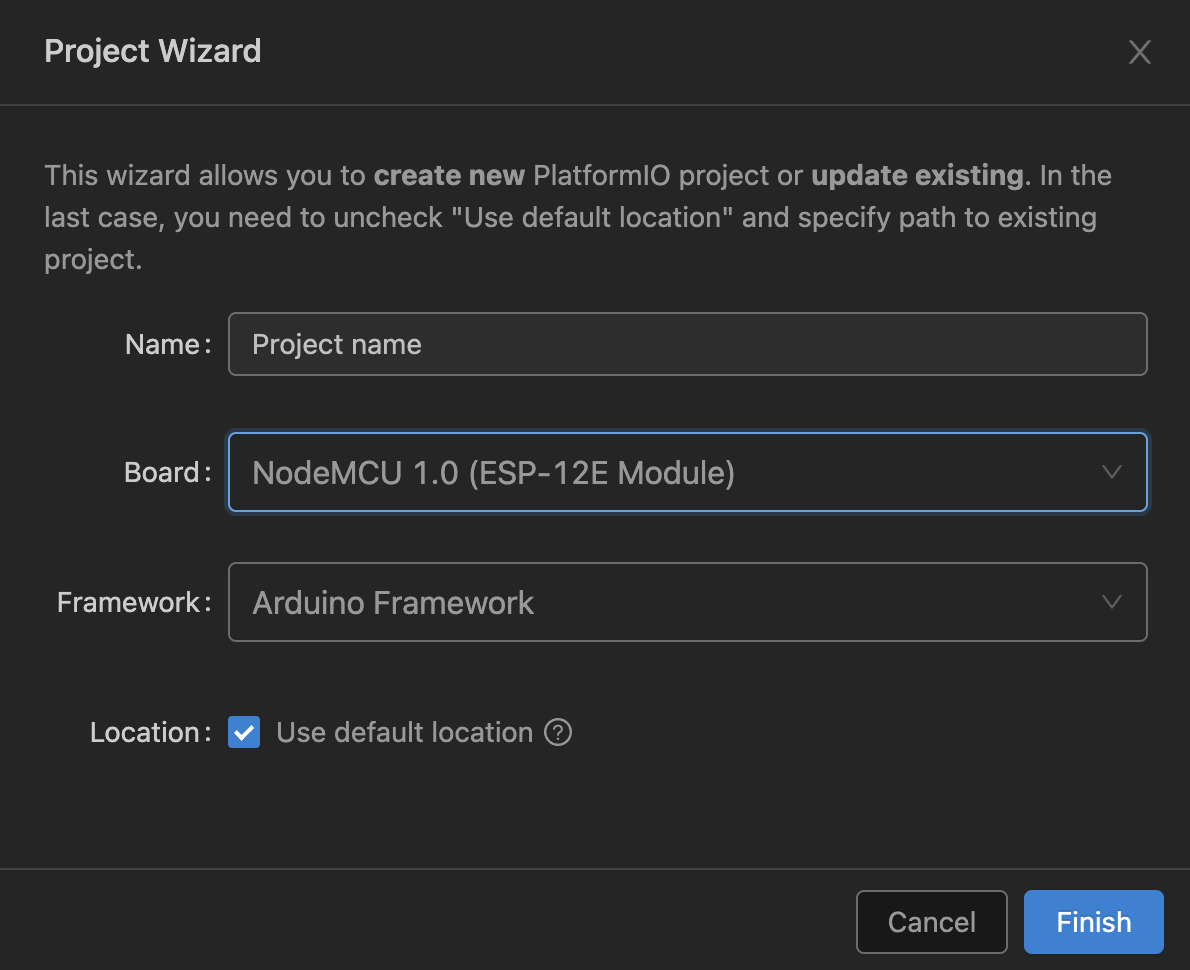
\includegraphics[scale=0.6]{resources/platformio-new-project}
		\caption{Меню создания нового проекта в PlatformIO}
		\label{fig4.1}
	\end{figure}
	
	Первым шагом при программировании микроконтроллера стало создание проекта при помощи PlatformIO.
	На этапе создания нового проекта появляется возможность выбора контроллера. Основными составляющими
	в проекте являются конфигурационный файл platformio.ini, в котором указывается модель контроллера,
	а также подключаемые к проекту библиотеки, и директива src, в которой должен содержаться код проекта.
	
	При первоначально настройке в папке src содержится единственный файл main.cpp. Он включает два
	метода. Метод setup() отвечает за первоначальную конфигурацию контроллера, а метод loop()
	повторяется всё время, пока контроллер подключен к питанию.
	
	Для знакомства с программированием данного типа контроллеров и изучения программных методов
	было реализовано несколько базовых примеров. Первым из них было мигание встроенного на контроллере
	индикатора. Затем были построены простейшие схемы с использованием макетной платы, диода и
	нескольких проводов. Мигание встроенного индикатора было заменено миганием диода. После этого
	был реализован пример управления диода по нажатию кнопки. Наконец, был задействован Wi-Fi модуль
	для управления диодом с компьютера. Данный пример был взят за основу практического прототипа. Более
	подробно работа прототипа и все этапа обмена сообщениями будут рассмотрены позже. Но перед этим
	перейдём к криптографической части данной работы.
	
	\begin{figure}[h]
		\centering
		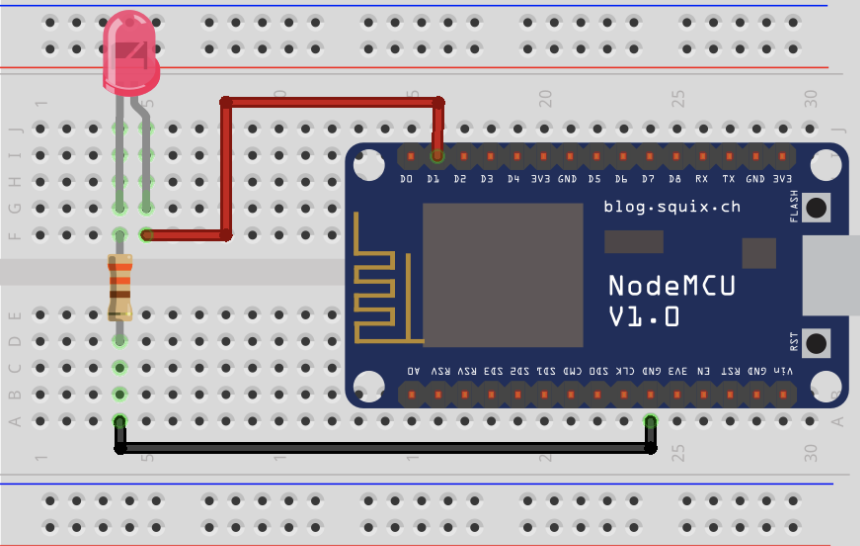
\includegraphics[scale=0.6]{resources/esp8266-control-led}
		\caption{Схема подключения диода к микроконтроллеру}
		\label{fig4.2}
	\end{figure}
	
	
	\section{Реализация и использование криптографического стандарта СТБ 34.101.77}
	
	\subsection{Описание стандарта}
	
	Официальное название стандарта $-$ <<Криптографические алгоритмы на основе sponge-функции>> \cite{standard-77}.
	Разберём для начала, что из себя представляет sponge-функция.
	
	Sponge-функция $-$ это класс алгоритмов с конечным внутренним состоянием. Эти алгоритмы
	предназначены для обеспечения конфиденциальности, целостности и подлинности информации
	при её передачи и обработке. Сама функция задаёт сложное преобразование двоичных слов большой 
	длины. Криптографические алгоритмы подразделяются на две большие группы:
	
	\begin{enumerate}
		\item алгоритмы хэширования, описанные в разделе 7 стандарта;
		\item программируемые алгоритмы, описанные в разделе 8.
	\end{enumerate}

	В практической части данной работы используются только программируемые алгоритмы, в частности
	алгоритмы аутентифицированного шифрования, которые представляют собой последовательности 
	команд криптографического автомата. Более подробно о них речь пойдёт далее.

	Стандарт описывает преобразование двоичных слов длины 1536 бит (192 байта). Преобразование
	задаётся алгоритмом bash-f, который в свою очередь использует алгоритм bash-s. bash-f и bash-s
	являются sponge-функциями, которые определяют программируемые алгоритмы. Стандартные уровни
	стойкости $l = 128, 192, 256$. Дополнительным параметром является ёмкость $d \in \{1, 2\}$.
	В программируемых алгоритмах также используется ключ $K$, длина которого должна быть не меньше 
	уровня стойкости, но также не превосходить 480. Для контроля целостности и подлинности вычисляется
	имитовставка, длина которой равна уровню стойкости $l$.
	
	Управление автомата, лежащего в основе программируемых алгоритмов, осуществляется командами.
	Допустимы следующие команды:
	
	\begin{itemize}
		\item start (инициализация). На этом этапе происходит загрузка ключа;
		\item restart (повторная инициализация);
		\item absorb (загрузка данных);
		\item squeeze (выгрузка данных). С помощью этой команды осуществляется вычисление имитовставки;
		\item encrypt (операция зашифрования);
		\item decrypt (операция расшифрования);
		\item ratchet (необратимое изменение состояния автомата);
		\item commit (подтверждение выполнения других комманд).
	\end{itemize}

	В практической части данной работы были реализованы команды start, absorb, squeeze, encrypt, 
	decrypt, commit. Все перечисленные команды используются в аутентифицированном шифровании,
	которое и применяется для защиты данных, передаваемых между умными устройствами. Алгоритм
	установки защиты заключается в последовательном применении команд start, absorb, encrypt, squeeze,
	а алгоритм снятия защиты выполняет команды start, absorb, decrypt и squeeze соотвественно.
	
	\subsection{Практическая реализация}
	
	Алгоритмы bash-s и bash-f являются низкоуровневыми, поскольку оперируют с битами. Поэтому они 
	были реализованы на языке программирования C. Так как язык прошивки микроконтроллера $-$ C++,
	а язык клиентского приложения $-$ Java, команды для управления автоматом при аутентифицированном 
	шифровании необходимо было реализовать на двух этих языках. Рассмотрим сначала реализацию на Java.
	
	Практически во всех командах используется алгоритм bash-f, в связи с чем возникла необходимость
	вызова нативного C кода из программы на Java. Для этого используется технология JNI (Java 
	Native Interface). Однако перед этим необходимо скомпилировать код на C в динамическую библиотеку.
	Рассмотрим более детально шаги для вызова нативного кода из программы на Java:
	
	\begin{enumerate}
		\item Для начала нужно создать Java класс с методом, объявленным как native:
		\begin{lstlisting}
			class LibraryNative {
				public static native byte[] bash_f(byte[] array);
			}
		\end{lstlisting}
		\item После этого скомпилировать файл с опцией -h для генерация header-файла:
		\begin{lstlisting}[language=Bash]
			javac LibraryNative.java -h .
		\end{lstlisting}
		\item Создать файл LibraryNative.c. Скопировать определение метода из файла LibraryNative.h
		и добавить реализацию:
		\begin{lstlisting}[language=C]
			#include <jni.h>
			#include <inttypes.h>
			#include <string.h>
			#include "LibraryNative.h"
			
			JNIEXPORT jbyteArray JNICALL Java_LibraryNative_bash_1f(JNIEnv *env, jclass thisClass, jbyteArray inJNIArray) {
				// insert implementation here
			}
		\end{lstlisting}
		\item Сгенерировать динамическую библиотеку. Практическая часть данной работы выполнены на 
		операционной системе MacOS, поэтому генерируется файл с расширением .dylib:
		\begin{lstlisting}[language=Bash]
			gcc -I"$JAVA_HOME/include" -I"$JAVA_HOME/inc lude/darwin" -dynamiclib -o libLibraryNative.dylib LibraryNative.c
		\end{lstlisting}
		\item Запустить метод из программы на Java, предварительно загрузив библиотеку в явном виде:
		\begin{lstlisting}
			public class Runner {
				
				static {
					System.loadLibrary("LibraryNative");
				}
			
				public static void main(String[] args) {
					LibraryNative.bash_f(new byte[192]);
				}
			}
		\end{lstlisting}
	\end{enumerate}

	Далее были реализованы команды, а также методы для установки и снятия защиты в аутентифицированном 
	шифровании строго в соответствии со стандартом.
	
	Реализация стандарта на C, как и других белорусских криптографических стандартов, содержится 
	в библиотеке bee2. Проблема заключается в несовместимости этой библиотеки с платформой PlatformIO,
	на базе которой написана прошивка для микроконтроллера. В связи с этим возникла необходимость
	реализовать часть стандарта, ответственную за шифрование, самостоятельно. За основу была взята
	имплементация из библиотеки bee2.
	
	Также в коде были реализованы юнит тесты с данными из приложения А соответствующего стандарта для
	верификации корректности реализации алгоритмов и команд.

	
	\section{Модель прототипа}
	
	Результатом работы над практической частью является реализация протокола взаимодействия между
	двумя умными устройствами с применением белорусского криптографического стандарта. Протокол
	включает в себя защищённый обмен сообщениями. Рассмотрим более детально взаимодействие конечного
	устройства (умной лампочки на базе микроконтроллера ESP8266) и управляющего устройства (компьютера).
	
	На этапе присоединения конечное устройство подключается к сети Wi-Fi, в которой уже находится
	управляющее устройство. После этого на конечном устройстве запускается упрощённый веб-сервер
	(с выделенным статическим IP адресом),
	который ожидает команды от управляющего устройства. Клиент посылает HTTP POST запросы на
	включение или выключение лампочки по REST API. При этом конечное устройство принимает только 
	корректно зашифрованные запросы и не реагирует на все остальные.
	
	Для осуществления подключения умного устройства к Wi-Fi сети используется специализированная
	библиотека WiFiManager. Процесс подключения происходит по следующей схеме:
	
	\begin{enumerate}
		\item При запуске Wi-Fi модуль на микроконтроллере работает в режиме программной точки доступа
		с предварительно заданным именем сети и паролем.
		\item На управляющем устройстве (компьютере) необходимо подключиться к соответствующей Wi-Fi сети, 
		после чего откроется страница со всеми доступными Wi-Fi сетями.
		\item В списке необходимо выбрать нужную сеть и ввести пароль.
		\item С этого момента умное устройство будет находится в выбранной сети в качестве Wi-Fi клиента.
	\end{enumerate}

	Описанные действия необходимо осуществить единожды $-$ при первом подключении устройства в сеть.
	В дальнейшем контроллер будет подключаться к сети автоматически при её наличии в зоне доступа.
	
	\begin{figure}[H]
		\centering
		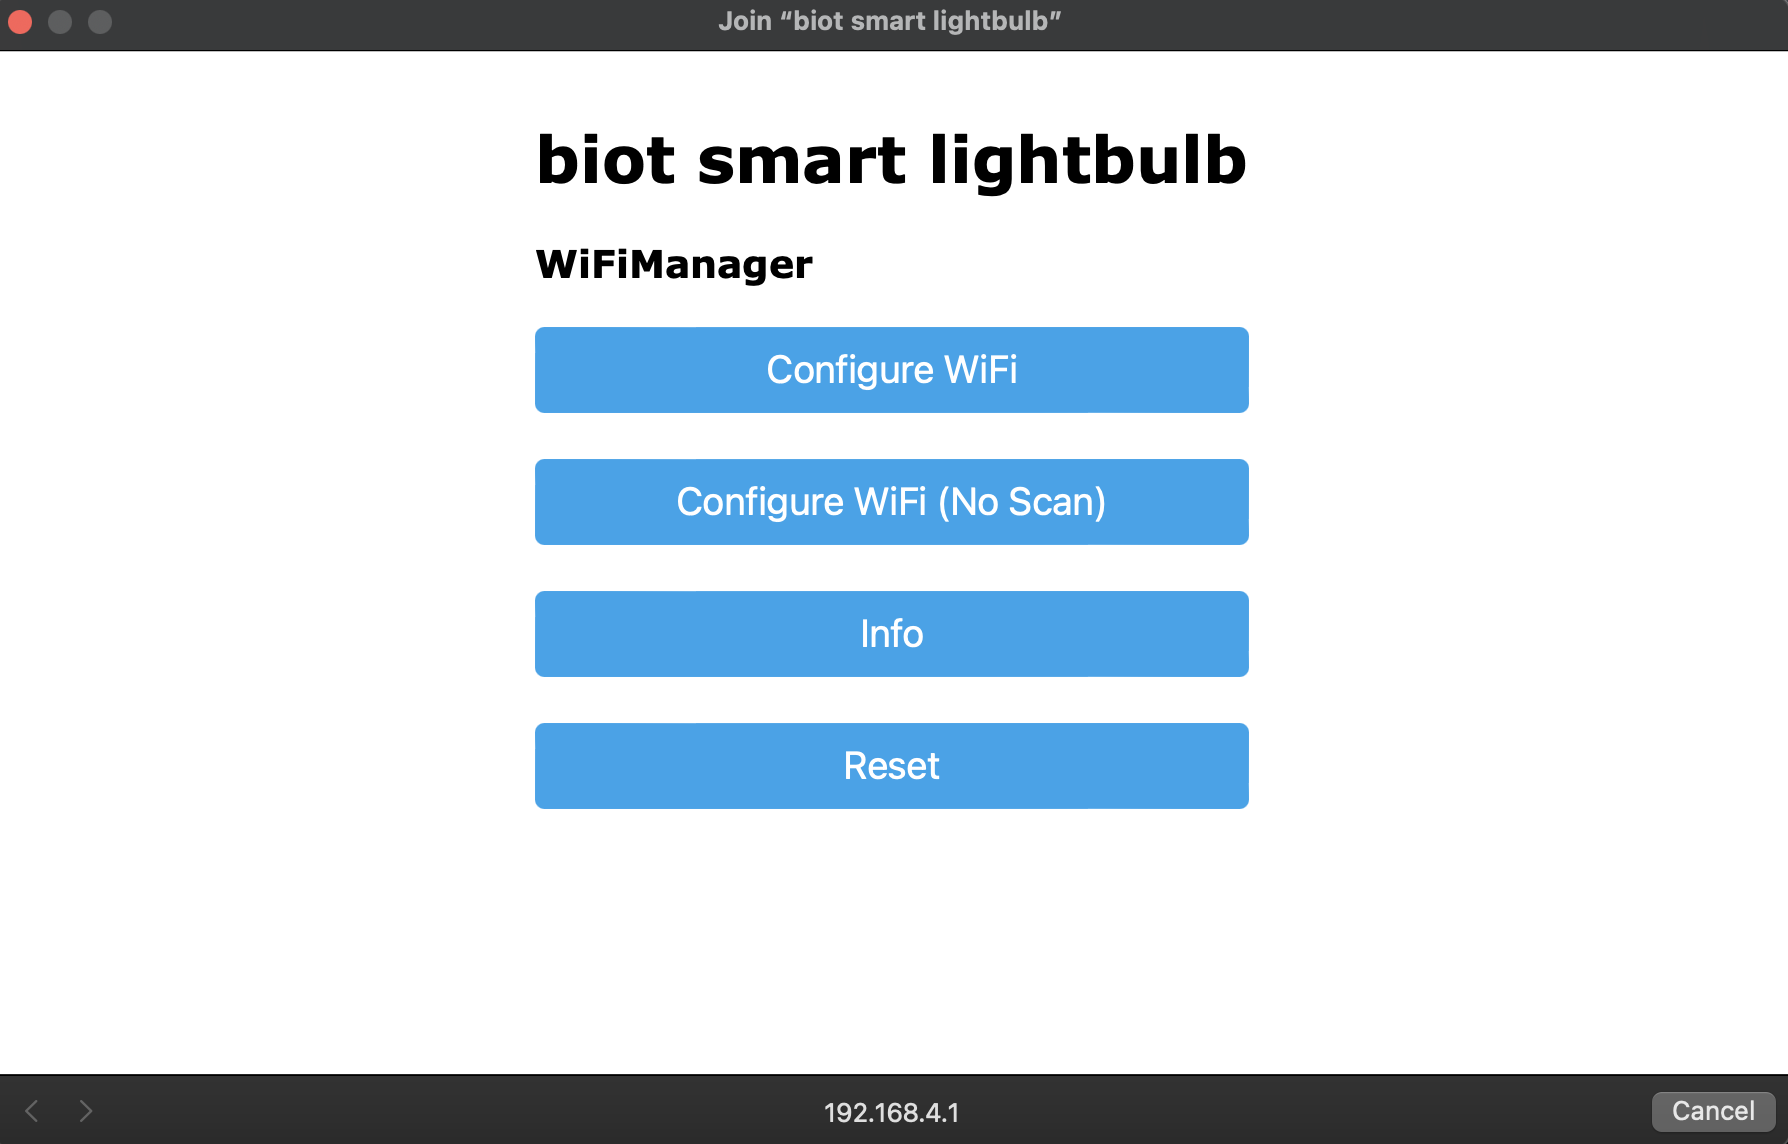
\includegraphics[scale=0.5]{resources/wifi-manager-1}
		\caption{Меню подключения умного устройства к Wi-Fi сети}
		\label{fig4.3}
	\end{figure}

	
	
	% добавить информацию о распределение ключа шифрования
	
			
	\chapter*{Заключение}
	\addcontentsline{toc}{chapter}{Заключение}
	
	Интернет вещей всё глубже проникает в жизнь конечного потребителя, набирая всё большую популярность.
	В связи с этим вопросы обеспечения безопасности конечных устройств и криптографической защиты данных
	пользователей остаются открытыми и актуальными.
	
	В первой главе текущего исследования были описаны ключевые технологии, применимые в IoT. Основными
	технологическими уровнями являются программное и аппаратное обеспечение, уровень коммуникации
	между устройства и платформа, которая их объединяет. Среди большого разнообразия используемых
	протоколов были выбраны три основных решения: ZigBee, Z-Wave, Wi-Fi $-$ и проведён сравнительный анализ
	их технических характеристик.
	
	Вторая глава продолжает описание и сравнение выбранных протоколов уже с точки зрения безопасности.
	Были рассмотрены алгоритмы выработки и распределения ключей, шифрования и контроля целостности
	данных, используемые в протоколах.
	
	Третья часть рассказывает об угрозах, свойственных сетям на основе ZigBee, Z-Wave и Wi-Fi, а также
	содержит описание успешно проведённых атак, с целью выявления уязвимостей и дальнейшего их
	устранения. В соответствии с поставленными во введении целями была построена матрицы угроз,
	которая отображает потенциальную уязвимость IoT протоколов к определённым типам криптографических 
	атак. В качестве набора базовых угроз были выбраны следующие: атака <<человек посередине>>,
	атака повторного воспроизведения, защита от <<чтения назад>>, атака понижения версии.
	
	В заключительной главе приведено описание процесса разработки прототипа, выбора технологий,
	обзор белорусского криптографического стандарта СТБ 34.101.77, мотивация использования
	и реализации аутентифицированного шифрования из этого стандарта. Также были детально описаны
	ключевые технические особенности разработанного решения, такие как установка соединения,
	выработка и распределение ключей шифрования, реализация счётчика отправленных и полученных
	сообщений.  Код прошивки для умного устройства, а также ключевых компонентов приложения
	для управляющего устройства приведен в приложениях к данной работе.
	
		 
	\newpage
 	
	 \begin{thebibliography}{1}
	 	\addcontentsline{toc}{chapter}{Список использованных источников}
	 	
	 	\bibitem{zigbee-certified-products} List of ZigBee certified products. -Mode of access: 
	 	\newline https://zigbeealliance.org/product\_type/certified\_product/. -Date of access: 11.12.2021.
	 	
	 	\bibitem{zigbee-alliance} ZigBee Alliance. -Mode of access: 
	 	\newline https://zigbeealliance.org/solution/zigbee/. -Date of access: 11.12.2021.
	 	
	 	\bibitem{z-wave-certified-products} List of Z-Wave certified products. -Mode of access: 
	 	\newline https://products.z-wavealliance.org. -Date of access: 11.12.2021.
	 	
	 	\bibitem{z-wave-alliance} Z-Wave Alliance. -Mode of access: 
	 	\newline https://z-wavealliance.org/. -Date of access: 11.12.2021.
	 	
	 	\bibitem{wi-fi-alliance} Wi-Fi Alliance. -Mode of access: 
	 	\newline https://www.wi-fi.org/. -Date of access: 11.12.2021.
	 	
	 	\bibitem{802.11-2016} 802.11-2016 - IEEE Standard for Information technology. -Mode of access: 
	 	\newline https://ieeexplore.ieee.org/document/7786995. -Date of access: 11.12.2021.
	 	
	 \end{thebibliography}	 
	
\end{document}